After virtual-channel allocation assigns an output port and an output virtual channel to a packet, each flit of the packet still needs to obtain permission to traverse the router switch. This permission is determined by the switch allocator. In each cycle, the switch allocator selects the input flits that are allowed to access the crossbar and generates the corresponding switch control signals.

The switch allocation process follows the same separable input-first idea introduced earlier. Each input port first arbitrates among its local virtual channels and selects at most one flit that is ready to move forward. As a result, only one request from each input port can be sent to the output side in a cycle. The selected requests are then grouped according to their target output ports. If several input ports request the same output port, the output-side arbiter grants only one of them. The winning input-output pair is then used to configure the crossbar traversal path for that cycle. Figure~\ref{fig:switch_allocation_flow} summarizes the overall switch allocation procedure.

Credit availability is also considered before a flit is allowed to participate in switch allocation. A flit is considered ready only if its assigned downstream virtual channel has available buffer space. When a flit is successfully selected and moves forward, the corresponding credit is consumed. Therefore, switch allocation is not only responsible for crossbar scheduling, but also works together with credit-based flow control to avoid sending flits into a full downstream buffer.

Overall, switch allocation determines the cycle-by-cycle movement of flits through the router. It ensures that each input port sends at most one flit and each output port receives at most one flit in a cycle, while maintaining correct backpressure behavior through credit checking.

\begin{figure}[htbp]
    \centering
    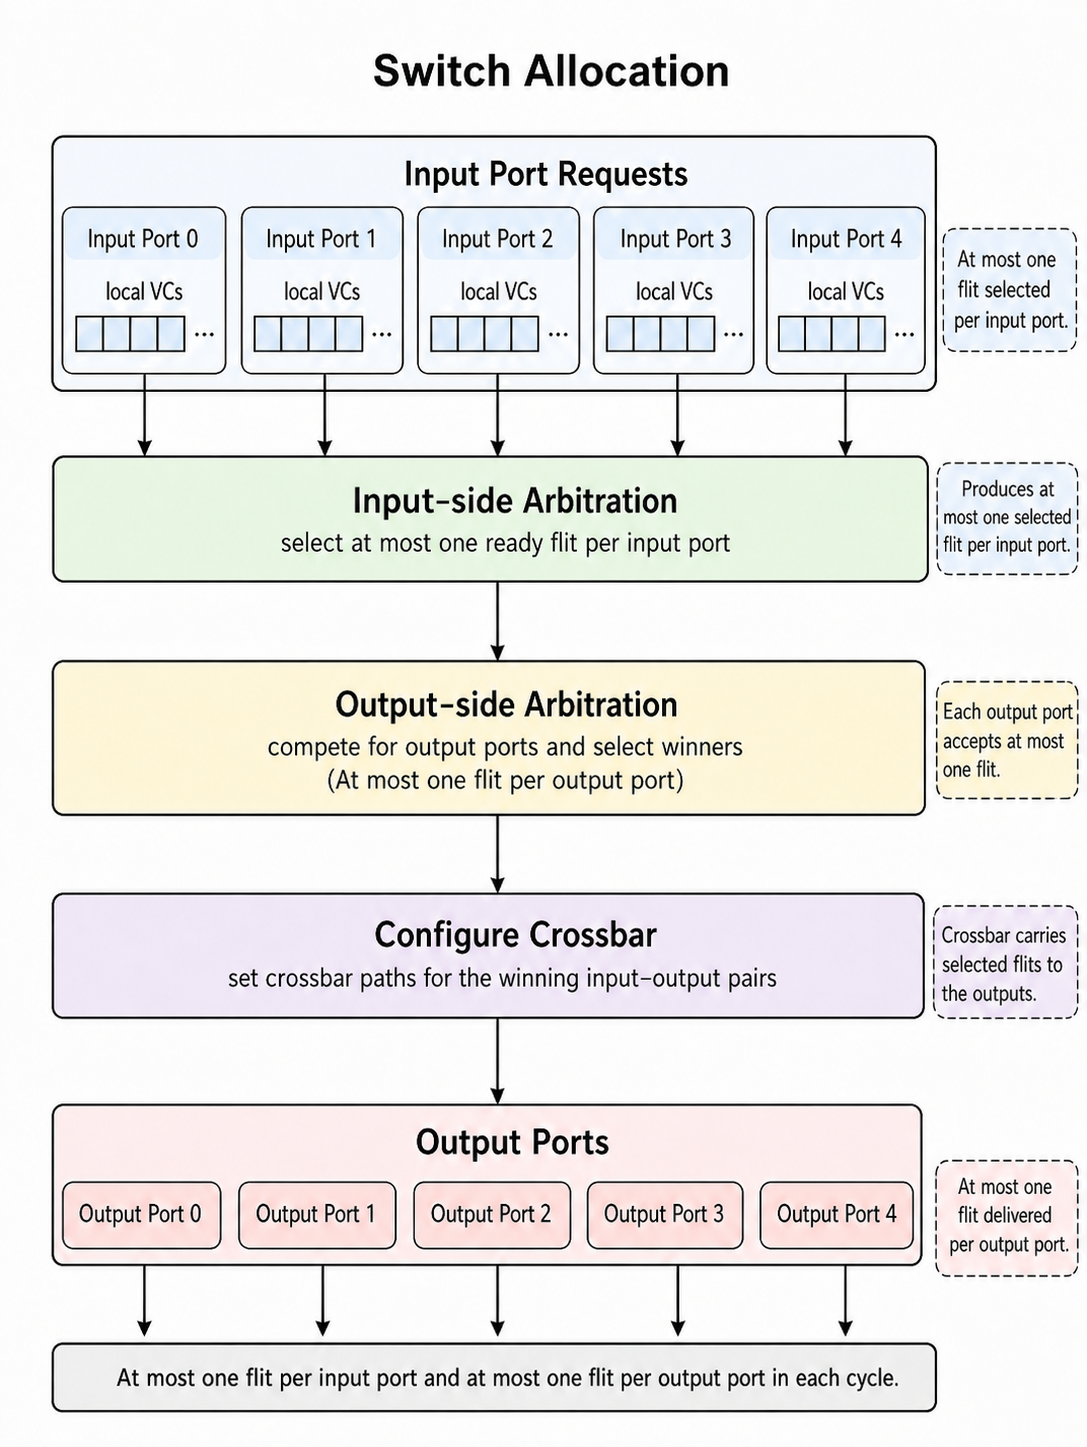
\includegraphics[width=0.6\textwidth]{images/ch3_design_and_implementation/switch_allocation.png}
    \caption{Switch allocation flow}
    \label{fig:switch_allocation_flow}
\end{figure}
